%% ------------------------------------------------------------------------- %%
\chapter{Desenvolvimento Guiado por Testes}
\label{cap:tdd}

Métodos ágeis de desenvolvimento de software focam em constante
\textit{feedback}, seja ele da equipe em relação ao cliente, seja da
qualidade (interna e externa) do código produzido à equipe \cite{AgileManifesto}.
Com isso, muitas das práticas sugeridas por métodos ágeis visam aumentar a 
quantidade e a qualidade desse \textit{feedback}; a ideia da programação pareada, por
exemplo, é dar \textit{feedback} sobre o código durante sua escrita.

Desenvolvimento Guiado por Testes (TDD), prática popularizada por Kent Beck por meio de seu livro
\textit{TDD: By Example} em 2001 \cite{TDDByExample}, é mais uma das práticas
ágeis na qual o foco é dar \textit{feedback}. TDD tem grande importância durante o ciclo
de desenvolvimento uma vez que, conforme sugerido pelas práticas ágeis, o projeto de classes de um
software deve emergir à medida que o software cresce. E, para responder
rapidamente a essa evolução, é necessário um constante \textit{feedback} sobre a
qualidade interna e externa do código.

TDD é uma prática de desenvolvimento de software que se baseia na repetição de
um pequeno ciclo de atividades. Primeiramente, o desenvolvedor escreve um
teste que falha. Em seguida, o faz passar, implementando a
funcionalidade desejada. Por fim, refatora o código para remover qualquer
duplicação de dados ou de código gerada pelo processo.
Além disso, simplicidade deve ser também algo intrínseco ao processo; o praticante
busca escrever o teste mais simples que falhe e escrever a implementação mais simples
que faça o teste passar.
Esse ciclo
é também conhecido como 
"Vermelho-Verde-Refatora" (ou \textit{"Red-Green-Refactor"}), uma vez que lembra as cores que um 
desenvolvedor normalmente vê quando faz TDD: o vermelho significa que
o teste está falhando, e o verde que o teste foi executado com sucesso.

Este capítulo aborda a prática de TDD, bem como cita
seus possíveis efeitos no processo de desenvolvimento de software, conforme relatado pela
literatura.

%% ------------------------------------------------------------------------- %%
\section{Benefícios de TDD}

Uma consequência da prática de TDD é a bateria de testes de unidade gerada.
A prática ajuda o programador a evitar erros de regressão, em que a implementação de
uma nova funcionalidade quebra uma outra funcionalidade já existente no sistema.
Essa bateria também provê segurança durante as
constantes refatorações de código que são feitas durante o processo de
desenvolvimento.
A quantidade de código coberto pelos testes também tende a ser alta, uma vez que o
desenvolvedor deve sempre escrever um teste antes de implementar uma nova
funcionalidade. 

É comum relacionar TDD à práticas de testes de software. No entanto, apesar de constar o
termo ``teste'' no nome, TDD não é visto apenas como uma prática de testes.
Embora a criação de testes seja algo intrínseco ao processo, é dito que TDD também 
auxilia o desenvolvedor a criar classes mais flexíveis, mais coesas e
menos acopladas. Os testes são a ferramenta que o programador utiliza para
validar o projeto de classes criado. Por esse motivo, muitos se referem a TDD como
\textit{Projeto de Classes Guiado por Testes} \cite{tdd-taxonomy}.

Autores como Kent Beck \cite{aim-fire}, Dave Astels \cite{astels-tdd} e
Robert Martin \cite{bob-martin} afirmam que TDD é, na verdade, uma prática de
projeto de classes \cite{tdd-taxonomy} \cite{aim-fire}.
Na opinião desses autores, a mudança na ordem do ciclo de
desenvolvimento tradicional, apesar de simples, agrega diversos outros
benefícios ao código produzido: maior simplicidade, menor acoplamento e maior
coesão das classes criadas, levando a um melhor projeto de classes, entre
outros. Ward Cunningham, um dos pioneiros da Programação Extrema, resume essa 
discussão em uma frase: \textit{"Test-First programming is not a testing technique"} 
que, em uma tradução livre, significa \textit{"Escrever primeiro os testes
não é uma prática de testes"}.

No entanto, é possível encontrar muitas definições que
não levam tal afirmação em conta. Algumas delas consideram apenas a ideia da
inversão da ordem de desenvolvimento, na qual o programador primeiro
escreve o teste e depois escreve o código que o faça passar.

Um exemplo é a definição que pode ser encontrada no livro \textit{JUnit
in Action} \cite{junit-in-action}: \textit{"Test-Driven Development é uma
prática de programação que instrui desenvolvedores a escrever código novo
apenas se um teste automatizado estiver falhando, e a eliminar duplicação. O
objetivo de TDD é 'código claro que funcione'"}.

Janzen levantou esse problema nas definições e comenta que um possível 
motivo é o próprio nome da prática, uma vez
que ela possui a palavra ``testes'', mas não contém a palavra \textit{``projeto''} 
\cite{tdd-really-improve}.
Segundo ele, uma definição mais clara é a de que TDD é a arte de produzir testes
automatizados para código de produção, usando esse processo para guiar o 
projeto e a programação \cite{agilealliance-tdd} \cite{tdd-taxonomy}.

%% ------------------------------------------------------------------------- %%
\section{Possíveis Efeitos no Projeto de Classes}

Como mencionado anteriormente, os praticantes de TDD acreditam que os testes de unidade
podem ajudá-los a criar um projeto de classes de qualidade. Uma das explicações mais
populares para esse fenômeno é a relação
entre um código que possui uma alta testabilidade, ou seja, é fácil de ser testado
por meio de um teste de unidade, e um projeto de classes de alta qualidade \cite{feathers-synergy}.

TDD também sugere que o programador dê sempre pequenos passos (conhecidos pelo termo em
inglês, \textit{baby steps}): deve-se escrever testes sempre para a menor
funcionalidade possível, escrever o código mais simples que faça o teste passar
e fazer apenas uma refatoração por vez \cite{TDDByExample}.
Uma justificativa para tal é a de que, quanto maior o passo que o programador dá, mais
tempo ele leva para concluí-lo e, consequentemente, ele fica mais tempo
sem \textit{feedback} sobre o código. Além disso, faz com que o programador não crie
soluções mais complexas do que elas precisam ser, tornando o código, a longo
prazo, o mais simples possível.

No entanto, apesar de muito ser dito sobre os efeitos de projeto de classes, e alguns deles
até serem demonstrados em estudos (conforme citado na Seção \ref{cap:trabalhos-relacionados}), 
pouco se sabe como a prática realmente influencia os desenvolvedores no momento da criação do
projeto das classes.

Para que possamos definir o que esperamos de um projeto de classes,
discutimos no Apêndice \ref{ape:design}
bons príncipios de projeto de classes orientados a objetos, que serão utilizados
na avaliação dos códigos produzidos pelos participantes deste estudo.

%% ------------------------------------------------------------------------- %%
\section{Trabalhos Relacionados}
\label{cap:trabalhos-relacionados}

Muitos estudos empíricos já foram realizados para avaliar os efeitos de TDD.
Em grande parte deles, os possíveis efeitos da prática no projeto de classes não é 
levado em conta, e apenas os efeitos da prática na qualidade externa são medidos.
Além disso, diferentemente
do que esta pesquisa propõe, muitos desses estudos optaram por um
maior controle no experimento, e os realizaram dentro de ambientes acadêmicos 
com estudantes dos mais diversos cursos de computação.

Janzen \cite{janzen-arch-improvement} mostrou que programadores que usam TDD na 
indústria produziram código que passaram em, aproximadamente, 50\% mais testes 
caixa-preta do que o código produzido por grupos de controle que não usavam TDD.
O grupo que usava TDD gastou menos tempo depurando. Janzen também 
apontou que a complexidade dos algoritmos era muito menor e a quantidade e
cobertura dos testes era maior nos códigos escritos com TDD.

Outros trabalhos realizados na indústria também apresentam resultados parecidos.
Um estudo feito por Maximillien e Williams \cite{max-e-williams} mostrou uma
redução de 40-50\% na quantidade de defeitos e um impacto mínimo na
produtividade quando programadores usaram TDD. Outro estudo feito por Lui e
Chan \cite{lui-e-chan} comparando dois grupos, um utilizando TDD e o outro 
escrevendo testes apenas após a implementação, mostrou uma redução  
no número de defeitos no grupo que utilizava TDD. 
Além disso, os defeitos que foram encontrados eram 
corrigidos mais rapidamente pelo grupo que utilizou TDD. O estudo feito por 
Damm \textit{et al.} \cite{damn-lundberg-e-olson} também mostra uma redução
em torno de 40\% a 50\% na quantidade de defeitos.

O estudo feito por George e Williams \cite{george-e-williams} mostrou que,
apesar de TDD poder reduzir inicialmente a produtividade dos desenvolvedores 
mais inexperientes, o código produzido passou entre 18\% a 50\% mais em testes 
caixa-preta do que códigos produzidos por grupos que não utilizavam TDD. Esse
código também apresentou uma cobertura de testes entre 92\% a 98\%. Uma análise
qualitativa mostrou que 87.5\% dos programadores acreditam que TDD facilitou o 
entendimento dos requisitos e 95.8\% acreditam que TDD reduziu o tempo gasto com
depuração. 78\% também acreditam que TDD aumentou a produtividade da equipe. 
Entretanto, apenas 50\% dos participantes disseram que TDD ajuda a diminuir o tempo de 
desenvolvimento. Sobre qualidade, 92\% pensam que TDD ajuda a manter um
código de maior qualidade e 79\% acreditam que ele promove um projeto de classes mais simples.

Turnu \textit{et al.} \cite{turnu-tdd-opensouce} discutem produtividade em
projetos de código aberto. Segundo eles, a produtividade caiu quando TDD foi
adotado completamente, mas em compensação o número de problemas diminuiu 
consideravelmente.

Nagappan \cite{nagappan-ms} conduziu estudos de caso na Microsoft e na IBM e os
resultados indicaram que o número de defeitos de quatro produtos diminuiu de 
40\% a 90\% em relação à projetos similares que não usaram TDD. Entretanto, o 
estudo mostrou também que TDD aumentou o tempo inicial de desenvolvimento entre 15\%
a 35\%. Langr \cite{langr} apontou que TDD aumenta a qualidade código, provê uma 
facilidade maior de manutenção e ajuda a produzir 33\% mais testes comparados  a
abordagens tradicionais.

Um estudo feito por Erdogmus \textit{et al.} \cite{erdogmus-morisio} com 24 estudantes de
graduação mostrou que TDD aumenta a produtividade. Entretanto nenhuma diferença 
de qualidade no código foi encontrada.

Outro estudo feito por Janzen \cite{janzen-saiedian} com três diferentes grupos
de alunos (cada um deles usando uma abordagem diferente: TDD, testes depois, sem
testes), mostrou que o código produzido pelo time que fez TDD usou melhor os
conceitos de orientação a objetos e as responsabilidades foram separadas em 13 
diferentes classes, enquanto os outros times produziram um código mais
procedural. O time de TDD também produziu mais código e entregou mais
funcionalidades. Os testes produzidos por esse time tiveram duas vezes mais
asserções que os outros e cobriram 86\% mais possíveis caminhos no código 
do que o time \textit{test-last}. 
As classes testadas tinham valores de acoplamento 104\% menor do 
que as classes não testadas e os métodos eram, na média, 43\% menos complexos 
do que os não-testados.

Dogsa e Batic \cite{dogsa-batic} também encontraram uma melhora no
projeto de classes feita com TDD. Mas, segundo os autores, essa melhora é 
consequência da simplicidade que a prática de TDD agrega ao processo. Eles
também  afirmaram que a bateria de testes de regressão gerada durante a prática 
possibilita ao desenvolvedor a constante refatoração do código.

Li \cite{angela-li} propôs um estudo qualitativo para
entender a eficácia de TDD. Por meio de um estudo de caso, ela coletou as 
percepções de benefícios que praticantes de TDD têm sobre a prática. Para isso ela
fez uso de cinco entrevistas semi-estruturadas realizadas em empresas de software de 
Auckland, Nova Zelândia. Os resultados das entrevistas foram analisados e alinhados
com os maiores temas discutidos sobre o assunto na literatura: qualidade de código,
qualidade da aplicação e produtividade do desenvolvedor.
No que diz respeito à qualidade de código, Li chegou a conclusão de
que TDD guia o desenvolvedor para classes mais simples e com melhor projeto de classes. 
Além disso, o código tende a ser mais simples e fácil de ler.
De acordo com o trabalho, os principais fatores que contribuem para esses benefícios
é a maior confiança em refatorar e modificar código, uma maior cobertura de testes,
entendimento mais profundo dos requisitos, maior facilidade na compreensão do código,
grau e escopo de erros reduzidos, além de uma maior satisfação pessoal do desenvolvedor.

O praticante de TDD geralmente faz uso também de outras práticas ágeis, como
programação pareada, o que pode dificultar o processo de avaliação dos benefícios
de TDD. Madeyski \cite{madeyski-package-dependencies} observou os resultados
entre grupos que praticavam TDD, grupos que praticavam programação pareada, 
e a combinação entre elas,
e não conseguiu mostrar grande diferença entre equipes que utilizam programação 
pareada e equipes que utilizam TDD, no que diz respeito ao gerenciamento de dependências entre 
pacotes de classes. Entretanto, ao combinar os resultados, Madeyski encontrou que TDD pode 
ajudar no nível de gerenciamento de dependências entre classes. Segundo ele, o 
programador deve utilizar TDD, mas ficar atento a possíveis problemas de projeto de classes.

O estudo de Muller e Hagner \cite{muller-e-hagner} apontou que TDD não resulta
em melhor qualidade ou produtividade. Entretanto, os estudantes avaliados perceberam um 
melhor reúso dos códigos produzidos com TDD. Steinberg \cite{steinberg} mostrou
que código produzido com TDD é mais coeso e menos acoplado. Os estudantes também
reportaram que os defeitos eram mais fáceis de serem corrigidos. A pesquisa feita
por Edwards \cite{edwards}, com 59 estudantes, mostrou que o código produzido com
TDD tem 45\% menos defeitos e faz o programador se sentir mais a vontade
com ele.

Aprender TDD também não é tarefa fácil. Mugridge \cite{mugridge} identificou
dois desafios principais em ensinar TDD: fazer os estudantes
pensarem novamente sobre o projeto de classes, e fazê-los se envolver com essa nova
abordagem. 
Contudo, segundo Proulx \cite{proulx}, a partir do momento em que
o estudante aprende TDD, ele tende a ter uma melhor performance em disciplinas
de orientação a objetos. Segundo ele, essa melhora é percebida inclusive pelos
empregadores desses alunos. 

Como os estudos discutidos acabam por misturar efeitos da prática de TDD na
qualidade externa e interna, a Tabela \ref{tab:comparativo} mostra
quais trabalhos apontaram efeitos no projeto de classes.

\begin{table}
	\centering
	\begin{tabular}{ | l | l | l |}
		
		\hline
		
		Possível Efeito & Tipo de Estudo & Trabalho\\

		\hline
		
		\multirow{2}{*}{Simplicidade}                          & Quantitativo & \cite{janzen-arch-improvement}, \cite{janzen-saiedian} \\
		                                           			   & Qualitativo  & \cite{angela-li}, \cite{george-e-williams}\\
		
		\hline
		
		Facilidade de manutenção                               & Quantitativo & \cite{langr}\\
		
		\hline
		
		\multirow{2}{*}{Melhor utilização de conceitos de orientação a objetos} & Quantitativo & \cite{janzen-saiedian}\\
		 													   & Qualitativo  & \cite{angela-li}, \cite{proulx}\\
		
		\hline
		
		Separação de responsabilidades                         & Quantitativo & \cite{janzen-saiedian}, \cite{steinberg}\\
		
		\hline
		
		Menor acoplamento                                      & Quantitativo & \cite{janzen-saiedian}, \cite{steinberg}\\
		
		\hline
		
		Maior reúso de classes                                 & Quantitativo & \cite{muller-e-hagner} \\

		\hline

	\end{tabular}
	\caption{Relação entre efeitos de TDD e estudos na literatura}
	\label{tab:comparativo}
\end{table}

Outras compilações de estudos sobre TDD também podem ser encontrados no livro
\textit{Test-Driven Development: An Empirical Evaluation of Agile Practice},
escrito por Madeyski \cite{madeyski-livro} ou no trabalho entitulado
\textit{Test driven development: empirical body of evidence}, feito por
Siniaalto \cite{tdd-body-of-evidence}.

%% ------------------------------------------------------------------------- %%
\subsection{Discussão}

Como apresentado, poucos trabalhos avaliam os efeitos de TDD sobre o
projeto de classes. Quando o fazem, apenas discutem quais os efeitos da prática
e não exatamente \textbf{como} TDD os influencia. Josefsson
\cite{josefsson}, em sua discussão sobre a necessidade de uma fase de projeto
arquitetural e os efeitos de TDD nesse quesito, chega à mesma conclusão. Segundo
ele, os estudos sobre TDD encontrados na literatura atual são muito limitados e
não são generalizáveis. Por esse motivo, os ditos efeitos que TDD têm 
sobre o projeto de classes não podem ser provados. Com base no levantamento
bibliográfico realizado, acreditamos que esta limitação se mantém.

Grande parte desses estudos também não levam em conta a experiência do
programador que está praticando TDD. Geralmente esse ponto é discutido apenas 
na seção de ameaças à validade do estudo. Janzen, em seu doutorado, percebeu que
desenvolvedores mais maduros obtêm mais benefícios de TDD, escrevendo classes
mais simples. Além disso, desenvolvedores maduros que experimentam a prática
tendem a optar por TDD mais do que desenvolvedores menos experientes
\cite{janzen-phd}.

Os trabalhos que analisam TDD do ponto de vista de projeto de classes, no entanto, não
chegam a resultados conclusivos; muitos deles dizem que os efeitos
de TDD não são tão diferentes daqueles dos times que não praticam TDD.  A própria tese de
doutorado de Janzen foi inconclusiva no que diz respeito à influência de TDD no 
acoplamento e na coesão \cite{janzen-phd}. 

Além disso, outro ponto fortemente relacionado com projeto de classes é a simplicidade e
facilidade de evolução. Um projeto de classes rígido, não favorável a mudanças,  é difícil de ser 
avaliado de maneira quantitativa. Complexidade
desnecessária também é totalmente subjetiva. 

Portanto, nossa crítica
com relação aos trabalhos relacionados é justamente na análise feita sobre os
efeitos da prática no TDD. É necessário mais do que uma comparação analítica; o
ponto de vista dos desenvolvedores, que atuam naquele código-fonte durante todo
o dia de trabalho deve ser levado em consideração.

%% ------------------------------------------------------------------------- %%
\subsection{Posição desta pesquisa na literatura atual}

Esta pesquisa se mostra diferente da maioria dos trabalhos encontrados na
literatura atual. Além de observar TDD pelo ponto de vista única e
exclusivamente do projeto de classes, colhe-se informações baseadas no ponto de
vista de desenvolvedores que a praticam.

Talvez o trabalho mais parecido com o que é proposto aqui é o
realizado por Angela Li, em 2009, que apresenta um estudo qualitativo sobre os
efeitos de TDD no processo de desenvolvimento de software \cite{angela-li}. 
A diferença é que esta pesquisa se concentra em entender os
efeitos de TDD no projeto de classes.
Além disso, diferentemente de outros trabalhos qualitativos, nossas entrevistas foram
abertas e totalmente focadas na criação do projeto de classes. Muitos argumentos interessantes
surgiram ao fazer o programador pensar melhor a respeito sobre o assunto.

O caminho em destaque da Figura \ref{fig:posicao-pesquisa} mostra a nossa posição
em relação ao que já é encontrado na literatura.

\begin{figure}[h!]
  \centering
  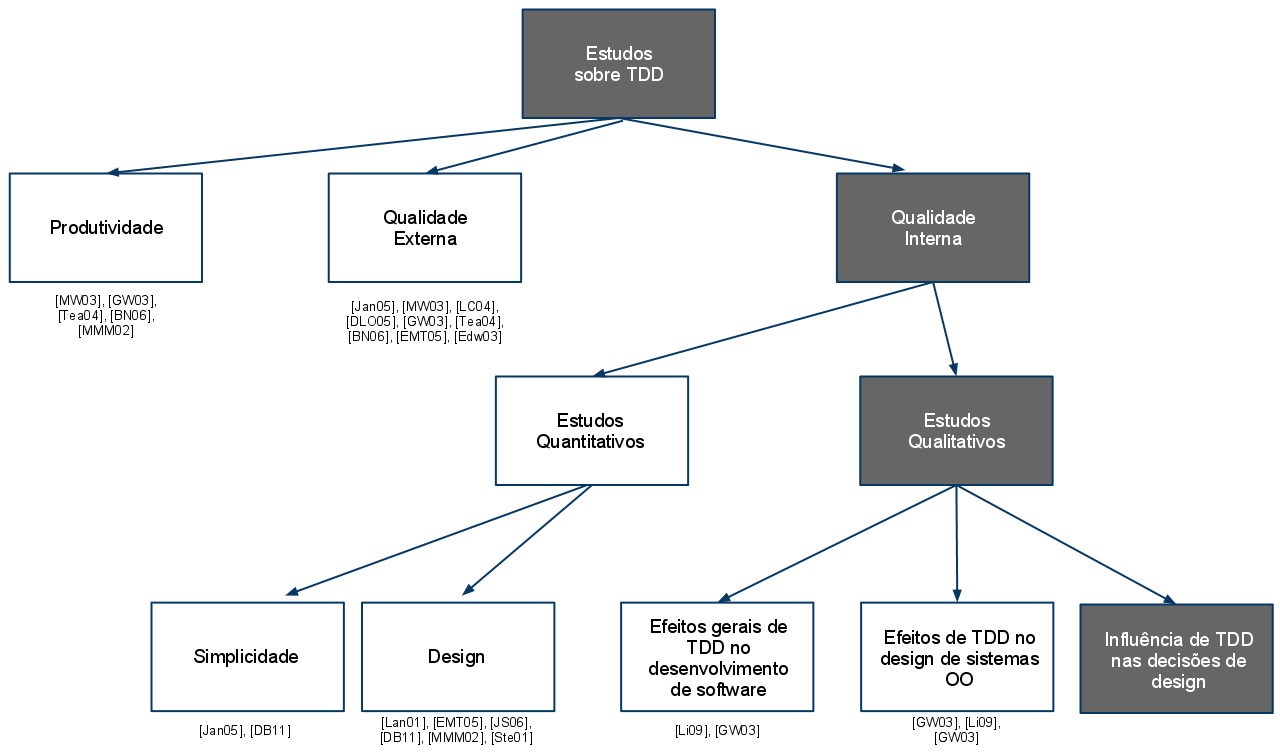
\includegraphics[scale=0.35]{posicao-pesquisa.png}
  \caption{Posição desta pesquisa na literatura atual}
  \label{fig:posicao-pesquisa}
\end{figure}

